\documentclass[11pt,letterpaper]{article}

\newenvironment{proof}{\noindent{\bf Proof:}}{\qed\bigskip}

\newtheorem{theorem}{Theorem}
\newtheorem{corollary}{Corollary}
\newtheorem{lemma}{Lemma} 
\newtheorem{claim}{Claim}
\newtheorem{fact}{Fact}
\newtheorem{definition}{Definition}
\newtheorem{assumption}{Assumption}
\newtheorem{observation}{Observation}
\newtheorem{example}{Example}
\newcommand{\qed}{\rule{7pt}{7pt}}

\newcommand{\solution}[4]{
\thispagestyle{plain} 
\newpage
\setcounter{page}{1}
\noindent
\begin{center}
\framebox{ \vbox{
\vspace{4mm}
\vspace{0.2in} 
{\centering \large\mbox{#3}}\\
\vspace{0.1in}
{#1 \hfill {Date: #2}}
}}
\end{center}
\markright{#1}
}

\newenvironment{algorithm}
{\begin{center}
\begin{tabular}{|l|}
\hline
\begin{minipage}{1in}
\begin{tabbing}
\quad\=\qquad\=\qquad\=\qquad\=\qquad\=\qquad\=\qquad\=\kill}
{\end{tabbing}
\end{minipage} \\
\hline
\end{tabular}
\end{center}}

\def\Comment#1{\textsf{\textsl{$\langle\!\langle$#1\/$\rangle\!\rangle$}}}



\usepackage{graphicx, amssymb, amsmath, listings, float, mathtools}
\usepackage{color, url}
\lstset{language = Python}
\lstset{breaklines}
\lstset{extendedchars=false}

\oddsidemargin 0in
\evensidemargin 0in
\textwidth 6.5in
\topmargin -0.6in
\textheight 9.0in

\begin{document}

\solution{\large Jifu Zhao}{\large 11/18/2016}{\bf \Large ECE 544NA \hspace{0.5cm} 
		Fall 2016 \hspace{0.5cm} Assignment 5}

\section*{\Large TensorFlow}

\subsection*{\large 1. Methods}

\begin{description}

\item[(1) ] In this assignment, we first implement the recurrent neural network in the format of basic RNN and LSTM. The input image has the dimension of $28 \times 28$, in this work, we can treat each pixel as one input, which has $784$ steps, or treat each column as one input, which has $28$ steps. Using basic RNN or LSTM, we finally get $4$ different models. The whole structure of the RNN class is shown in Figure \ref{fig:structure}.

\begin{figure}[H]
\centering
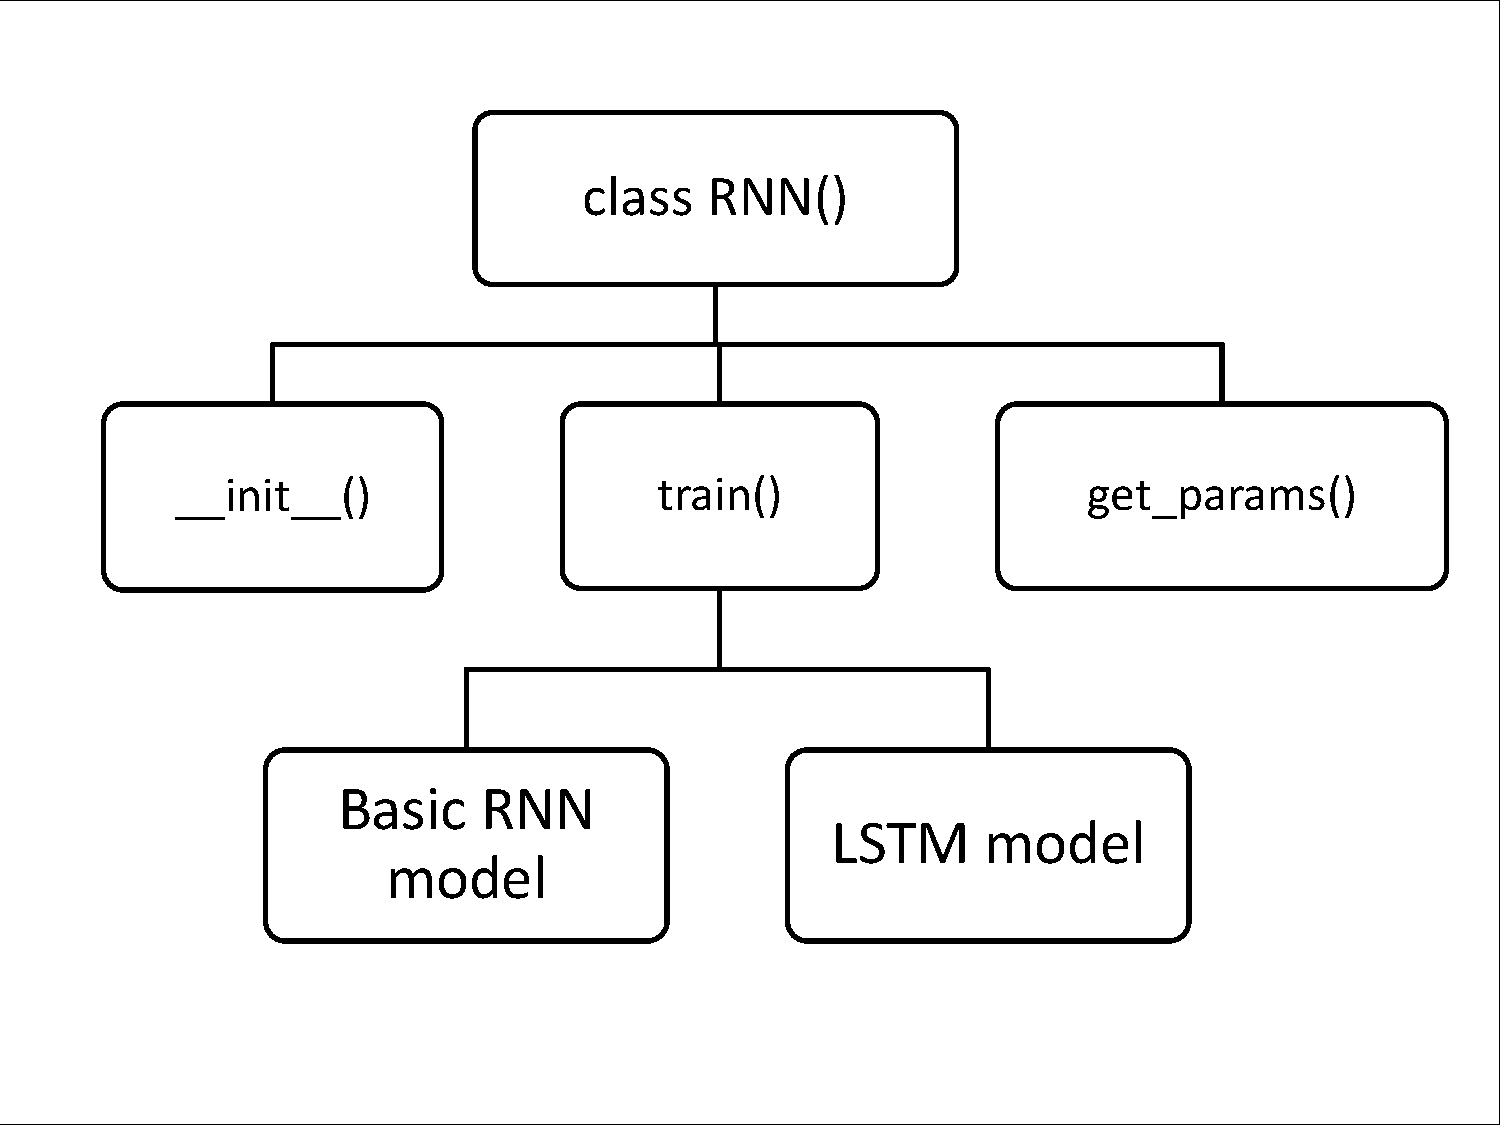
\includegraphics[width=0.8\textwidth]{./figures/ECE544hw5.pdf}
\caption{\label{fig:structure} Algorithm Structure}
\end{figure}

In class RNN(), after initialization using the function $\_\_init\_\_()$, the RNN model will be trained according to the given parameters using the function $train()$. In this process, the we will first create the so-called RNN cell using the function $tf.nn.rnn\_cell.BasicRNNCell()$ or $tf.nn.rnn\_cell.BasicLSTMCell()$ for basic RNN model or LSTM model. Then the RNN will be created using the function $ tf.nn.rnn(cell)$. The output from the RNN model has $100$ dimensions, and we will use a fully-connected neural network for the final classification problem, where the final output has $10$ dimensions. In this process, we find that when the final output is the linear connection rather than the softmax connection, the model trained much faster and the accuracy is also good. So, we choose linear activation function and using the cross-entropy as the loss function. Through using the Adam optimizer, we can train the overall model directly. Due to the size of the large dataset, we choose mini-batch learning method and finally evaluating the model on all the training set and testing set. \\

Note: In this section, we followed some online tutorials for RNN implementions, including:
	\begin{description}
	\item[a.]$https://www.tensorflow.org/versions/r0.11/tutorials/recurrent/index.html$
	\item[b.]$https://tensorhub.com/aymericdamien/tensorflow-rnn$
	\item[c.]$https://github.com/tflearn/tflearn/blob/master/examples/images/rnn\_pixels.py$
	\item[d.]$https://github.com/tensorflow/tensorflow/blob/master/tensorflow/g3doc/api_docs/\\
				python/functions_and_classes/shard0/tf.nn.rnn.md$
	\end{description}

\item[(2) ] Limited by the computation resources, we didn't train too many iterations, especially for the model with $784$ steps. The detailed parameter settings are listed in Table \ref{table:parameter}.
\begin{table}[H]
	\centering
	\caption{Parameter settings}
	\label{table:parameter}	
	\begin{tabular}{c | c | c | c | c}
		\hline \hline
		Model 		  &	Basic RNN (t=784) & LSTM (t=784) &	Basic RNN (t=28) & LSTM (t=28) \\[0.1cm]
		\hline
		steps size	  &	784			  &	784			 	 &	28			 	 & 28 	 	   \\[0.1cm]
		input size	  &	1			  &	1			 	 &	28			     & 28		   \\[0.1cm]
		learning rate &	0.0005		  &	0.0001		 	 &	0.0001 		     & 0.0001	   \\[0.1cm]
		iterations	  &	2000		  &	1000		  	 &	5000 		     & 5000        \\[0.1cm]
		batch size	  &	100			  &	100			 	 &	100			     & 100		   \\[0.1cm]
		\hline	
	\end{tabular}
\end{table}
\end{description}

\newpage
\subsection*{\large 2. Results}

\begin{description}

\item[(1) ] During the training process, in each iteration, we also record the mini-batch training accuracy. The convergence curves for mini-batch training-corpus accuracy of $4$ different models are shown in Figure \ref{fig:curve}.

\begin{figure}[H]
\centering
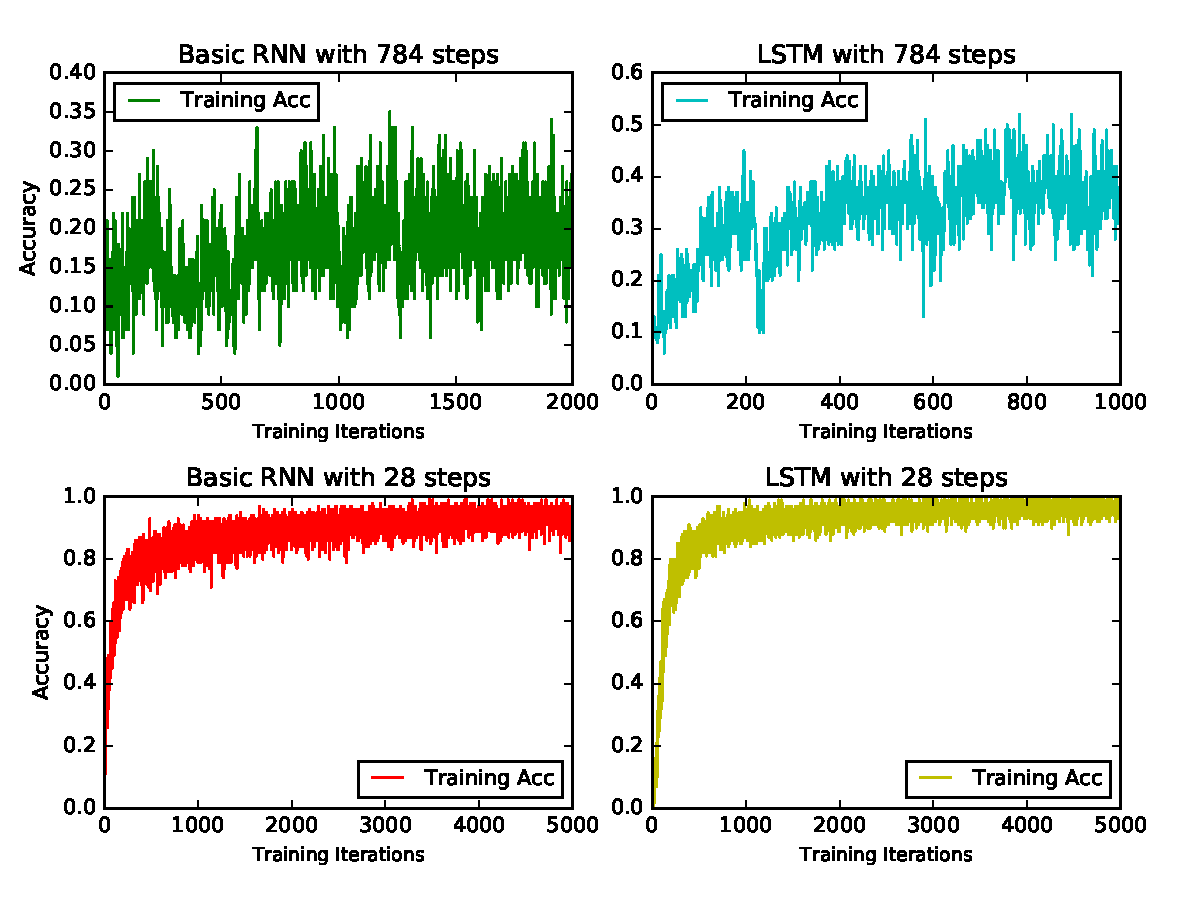
\includegraphics[width=0.97\textwidth]{./figures/convergence.pdf}
\caption{\label{fig:curve} Convergence Curve}
\end{figure}

Since the mini-batch is not very big ($100$ in this case), the learning curves for Basic RNN and LSTM with $784$ steps are not very smooth. But for $28$ steps case, both basic RNN model and LSTM model converge much better.

\item[(2) ] After finishing the iterations, we evaluate the model on the all training set and testing set. The final training and testing accuracy are shown in Table \ref{table:accuracy}

\begin{table}[H]
	\centering
	\caption{Training and testing accuracies}
	\label{table:accuracy}	
	\begin{tabular}{c | c | c }
		\hline \hline
		Model 				&	Training Set	&  Testing Set \\[0.1cm]
		\hline
		Basic RNN (t=784) 	&	20.40\%			&  20.95\%     \\[0.1cm]
		LSTM (t=784)		&	40.82\%			&  40.76\%     \\[0.1cm]   
		Basic RNN (t=28)	&	93.61\%			&  94.20\%     \\[0.1cm]
		LSTM (t=28)			&	96.68\%			&  96.51\%     \\[0.1cm]
		\hline	
	\end{tabular}
\end{table}

\end{description}


\clearpage

%\bibliographystyle{plain}
%\bibliographystyle{unsrt}
%\bibliography{reference.bib}

\end{document}

